\section{Batched Skip-Gram Model} \label{sec:contribution}
This section will give an overview of our implementation. The proposed implementation is a slighlty altered version of the origina Skip-Gram Model with negative sampling (SGNS). The idea behind this altering, is to compute the loss for multiple words and context pairs at the same time, this is inspired from mini-batch training, a model often used in other machine learning problem. Instead of computing the loss function of each pair, we computed the sum over a certain number of pairs (i.e 2000) as a loss. The exact process will be described in the following paragraph.
\subsection{Forwarding}
As the computation of the new loss function represents the challenging part of our implementation the forwarding method is explained step by step. Each time step is illustrated to make the explanation clearer.\\
Let $X = {(v_1,c_1),(v_2,c_2),(v_3,c_3)}$, be the training batch, where $(v_i,c_i)$ is a training sample constituted by a word and one of its context words. 
\subsubsection{Input}
The forwarding method will accept two vectors $v$ and $c$, and a matrix $A$ as an input. The first vector represents all the center words in a batch, the second one the context words. The Matrix represents the negative samples. The two vectors are of the same length, defined as $n$. The matrix must be of dimension $n \times k$, with $k$ being the number of negative samples per pair. This means the $i^{th}$ row will store the negative samples for the $i^{th}$ word context pair.\\
The input can be illustrated as follows: \\
$v = \begin{bmatrix}
v_1 & v_2 & v_3
\end{bmatrix}, c = \begin{bmatrix}
c1\\
c2\\
c3\end{bmatrix}$ and $A =
\begin{bmatrix}
k_{1,1} & k_{2,1} & k_{3,1}\\
k_{1,2} & k_{2,2} & k_{3,2}\\
k_{1,3} & k_{2,3} & k_{3,3}\\
\end{bmatrix}$\\

\subsubsection{Concatenation of samples}
The concatenation of the vector $c$ and the Matrix $A$ will result in a Matrix $\tilde{A}$, with:\\
$\tilde{A} = \begin{bmatrix}
c_1 & k_{1,1} & k_{2,1} & k_{3,1}\\
c_2 & k_{1,2} & k_{2,2} & k_{3,2}\\
c_3 & k_{1,3} & k_{2,3}& k_{3,3}\\
\end{bmatrix}$
\bigskip

\subsubsection{Embeddings}
Now it's necessary to access the word embeddings. For this purpose a Matrix $E_v$ of dimensionality $n \times d$ where $d$ is the dimension of our word embedding is created. $E_v$ stores the word embedding of the $i^{th}$ word from our input vector $v$ in it's $i^{th}$ row. The same is done for the other Matrix $\tilde{A}$. This will result in a $n \times k+1 \times d$ Array $E_c$. \\

$E_v = \begin{bmatrix}
\tilde{v_1}_1 & \ldots & \tilde{v_1}_d\\
\tilde{v_2}_1 & \ldots & \tilde{v_2}_d\\
\tilde{v_3}_1 & \ldots & \tilde{v_3}_d\\
\end{bmatrix}
$, where $\tilde{v_i} = \begin{bmatrix}
\tilde{v_i}_1 & \ldots & \tilde{v_i}_d \end{bmatrix}$ is the embedding of $v_i$. \\

$E_c = \begin{bmatrix}
\tilde{c_1 }& \tilde{k_{1,1}} & \tilde{k_{2,1}} \\
\tilde{c_2 }& \tilde{k_{1,2}}& \tilde{k_{2,2}} \\
\tilde{c_3 }&\tilde{ k_{1,3} }& \tilde{k_{2,3}}\\
\end{bmatrix}$,
where each entry of the matrix is a vector of dimension $d$\\

\subsubsection{Batch multiplication and negation of samples}
Now we need to compute the dot product of each word vector with its pair and the negative samples, exactly as done as in the original loss function of Mikolov et al. shown in Equation \ref{eq:obj_neg_samples}. For this task some definitions are necessary: let $A_j$ be the $j^th$ row of the matrix A, let $E_c(i,j)$ be the $d$ dimensional embedding of the word stored in $\tilde{A}(i,j)$. The dot product is computed with a so-called batch multiplication\footnote{Documentation: https://pytorch.org/docs/stable/torch.html\#torch.bmm} which will result in a matrix $S$ where $S(i,j) = E_c(i,j) \cdot {E_v}_j$. This will result in a $n\times k+1$ Matrix $S$. Now we only have to negate the last $k$ rows. The sum of each row represents the loss computed in Equation \ref{eq:obj_neg_samples}, for each word context pair.
Since computation time is too long with this approach the loss function is altered\\

$S = \begin{bmatrix}
\tilde{v_1} \cdot \tilde{c_1} & -\tilde{v_1} \cdot \tilde{k_{1,1}} & -\tilde{v_1} \cdot \tilde{k_{2,1}}& -\tilde{v_1} \cdot \tilde{k_{3,1}}\\
\tilde{v_2} \cdot \tilde{c_2} & -\tilde{v_2} \cdot \tilde{k_{1,2}} & -\tilde{v_2} \cdot \tilde{k_{2,2}} & -\tilde{v_2} \cdot \tilde{k_{3,2}}\\
\tilde{v_3} \cdot \tilde{c_3} &-\tilde{v_3} \cdot c_3 \tilde{k_{1,3}} & -\tilde{v_3} \cdot c_3 \tilde{k_{2,3}}&-\tilde{v_3} \cdot \tilde{k_{3,3}}\\
\end{bmatrix}$\bigskip

\subsubsection{Loss function}
Summing the matrix $S$ and multiplying it with $-1$ (to make the problem a minimizing problem) results in the loss for our entire batch. As some words may appear more than once in the batch this will more be an average of it than as with Mikolov et al. \citep{mikolov2} the exact update per pair. \\
L = $- \sum_{(i,j) \in k \times n} S(i,j) $\\

This finishes the description of our batched approach. 

\subsection{Distribution of word frequencies}
\subsubsection{Boxplot}
The quality of a batch is dependent on  the number of multiple appearances of words in the batch. The more frequently a word appears in a batch, the training quality of the word decreases. For this matter we chose to analyze the distribution of word frequencies. A box plot of the distribution, on the text8 dataset, can be found in Figure \ref{fig:boxplot_freq}. 
\begin{figure}[h]
\centering
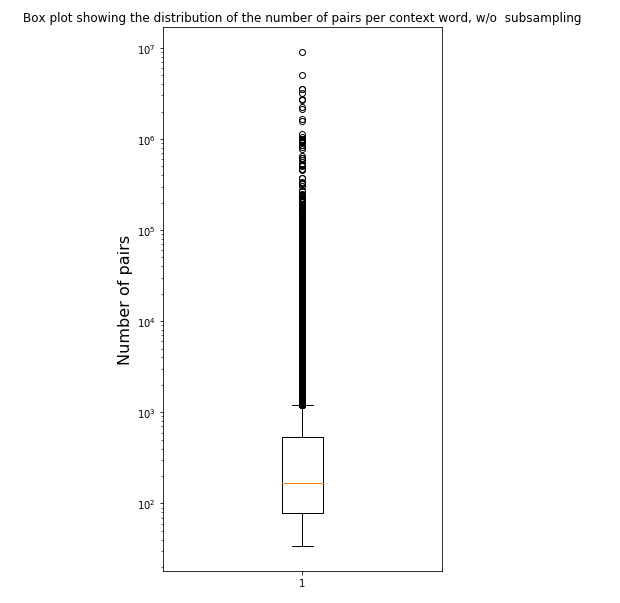
\includegraphics[scale=0.3]{images/no_sampling_boxplot}
\caption{Distribution of word frequencies in the text8 datasedt}
\label{fig:boxplot_freq}
\end{figure} 
This shows that very few words appear very frequently, and are therefore responsible for the building of the most context pairs. For example the word \textit{the} creates 50\% of the pairs in the text8 dataset. In consequence if we create arbitrary batches, most words  will appear multiple times in a batch and the learning will be hindered. A solution would be to only allow words to appear once in a batch, in the next section we present such a solution with a variable batch size. \subsubsection{Batches}
To solve this problem we only chose to block multiple appearance in a batch on the center words. The context words can be the same for two different center words.  Each batch will contain the highest possible number of pairs where each center word does not appear twice. The problem with this approach is that the batch size decreases very rapidly. This is due to the distribution of words. In consequence the average batch size is small and training time is increased, to remedy this problem we tried to reduce the number of very small batches, while maintaining the quality of learning. 
\subsubsection{Deletion of outliers}
To solve this matter, we looked again at the distribution of word frequencies (Figure \ref{fig:boxplot_freq}). We experimented with different settings (mean, median, average, outlier) and found that deleting all words that had a frequency greater than the 99\% was best. 
This technique drastically reduces the dataset size. 

The next section will describe our experimental setting and the possibilities that exists to evaluate the quality of word embeddings. 